% ======================================================================
%  Entrega 1 -- Modelos Estadisticos para la clasificacion y regresion
%  Informe: Parte 1 - Problema 1
% ======================================================================
\documentclass[10pt,a4paper]{article}

\usepackage[utf8]{inputenc}
\usepackage[T1]{fontenc}
\usepackage[spanish]{babel}
\usepackage[margin=1.5cm, top=1.3cm, bottom=1.3cm]{geometry}
\usepackage{booktabs}
\usepackage{amsmath}
\usepackage{xcolor}
\usepackage[hidelinks]{hyperref}
\usepackage{graphicx}



\definecolor{azul}{HTML}{1F5C9E}

% ======================================================================
\begin{document}
% ----------------------------------------------------------------------
% CARÁTULA
% ----------------------------------------------------------------------
\thispagestyle{empty}
\pagestyle{empty}

\begin{center}
\vspace*{1.5cm}

{\Large\bfseries\color{azul} Universidad de la República}\\[4pt]
{\large Facultad de Ingeniería}\\[2.5cm]


{\Large\bfseries\color{azul} Modelos Estadísticos para la}\\[-1pt]
{\Large\bfseries\color{azul} clasificación y regresión}\\[6pt]
{\large Entrega 1 --- Obligatorio}\\[3cm]

\textbf{Integrantes del grupo}\\[8pt]
\begin{tabular}{@{}lll@{}}
\toprule
\textbf{Nombre} & \textbf{Cédula} & \textbf{Correo}\\[1pt]
\midrule
Nombre Apellido 1 & 00.000.000-0 & \\
Nombre Apellido 2 & 00.000.000-0 & \\
Nombre Apellido 3 & 00.000.000-0 & \\
\bottomrule
\end{tabular}\\[3cm]

\textbf{Código del trabajo:} \url{https://github.com/usuario/repositorio}\\[2.5cm]


\textbf{Profesores:} 
\begin{center}
    María Inés Fariello\\[6pt]
    Gonzalo Cameto\\
\end{center}


\vfill

Montevideo, Uruguay\\[4pt]
Octubre de 2026

\end{center}

\newpage

\section{Problema 1}
\subsection{Simulación mediante aceptación-rechazo}

Se desea simular una muestra de tamaño $n$ de una variable aleatoria
cuya densidad es

\[
f_X(x;\theta) =
\frac{1}{2}(1+\theta x),
\qquad -1\leq x\leq1,
\]

tomando $\theta=-1/3$. Por lo tanto, la densidad considerada es

\[
f_X(x) =
\frac{1}{2}\left(1-\frac{x}{3}\right),
\qquad -1\leq x\leq1.
\]

Para generar la muestra se utiliza el método de aceptación-rechazo,
siguiendo el procedimiento presentado en el material del curso.

Como distribución propuesta se utiliza una uniforme en $[-1,1]$,
cuya densidad es

\[
g(x)=\frac{1}{2}.
\]

Se busca una constante $M$ tal que

\[
f_X(x)\leq M g(x).
\]

El máximo de $f_X$ se alcanza en $x=-1$, donde

\[
f_X(-1)=\frac{2}{3}.
\]

Por lo tanto,

\[
M=\frac{2/3}{1/2}=\frac{4}{3}.
\]

La probabilidad de aceptación de un candidato $x$ es entonces

\[
\frac{f_X(x)}{M g(x)}
=
\frac{3}{4}\left(1-\frac{x}{3}\right).
\]

El algoritmo consiste en generar un candidato $x\sim U(-1,1)$
y un valor $u\sim U(0,1)$. El candidato se acepta si

\[
u\leq
\frac{3}{4}\left(1-\frac{x}{3}\right).
\]

El procedimiento se repite hasta obtener $n$ observaciones aceptadas.\newline

La ejecución del programa resultó en lo siguiente:

\begin{verbatim}
Muestra final:
[ 0.05234615 -0.75480255 -0.70576528 -0.32312439  0.09243649  0.2595179
  0.76905297 -0.16095165  0.35687938 -0.18512842]

Aceptados:
[ 0.05234615 -0.75480255 -0.70576528 -0.32312439  0.09243649  0.2595179
  0.76905297 -0.16095165  0.35687938 -0.18512842]

Rechazados:
[0.17116325 -0.29715652]
\end{verbatim}

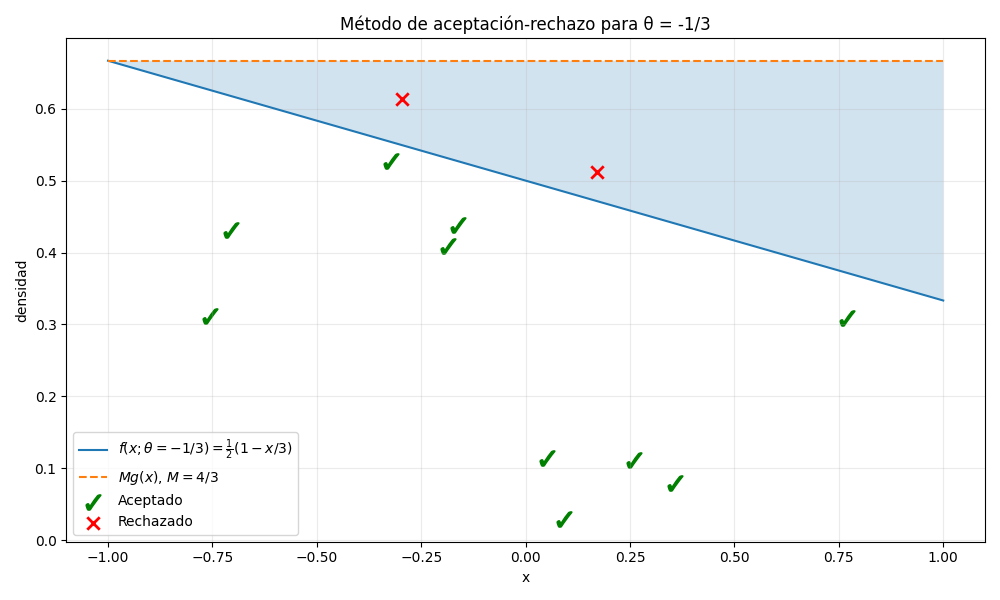
\includegraphics[width=0.8\textwidth]{../Imagenes/Prob1-1.png}

\newpage

\subsection{Estimador de máxima verosimilitud}

Sea $X_1,\ldots,X_n$ una muestra aleatoria de la distribución

\[
f_X(x;\theta)
=
\frac{1}{2}(1+\theta x),
\qquad -1\leq x\leq 1,
\qquad -1\leq\theta\leq1.
\]

Para una muestra de tamaño $n=10$, la función de verosimilitud está dada
por el producto de las densidades de las observaciones:

\[
V_{10}(\theta)
=
\prod_{i=1}^{10} f_X(x_i;\theta).
\]

Sustituyendo la expresión de la densidad:

\[
V_{10}(\theta)
=
\prod_{i=1}^{10}
\frac{1}{2}(1+\theta x_i).
\]

Por lo tanto,

\[
\boxed{
V_{10}(\theta)
=
\frac{1}{2^{10}}
\prod_{i=1}^{10}(1+\theta x_i)
}
\]

El estimador de máxima verosimilitud se define como el valor de
$\theta$ que maximiza la función de verosimilitud:

\[
\boxed{
\hat{\theta}
=
\underset{-1\leq\theta\leq1}{\operatorname{arg\,max}}
\ V_{10}(\theta)
}
\]

Como el logaritmo es una función monótona creciente,
maximizar la verosimilitud es equivalente a maximizar su logaritmo.

En este caso,

\[
\log V_{10}(\theta)
=
\log\left(
\frac{1}{2^{10}}
\prod_{i=1}^{10}(1+\theta x_i)
\right).
\]

Aplicando las propiedades del logaritmo:

\[
\log V_{10}(\theta)
=
-10\log(2)
+
\sum_{i=1}^{10}
\log(1+\theta x_i).
\]

Se considera el negativo del logaritmo de la verosimilitud:

\[
\ell_{10}(\theta)
=
-\log V_{10}(\theta).
\]

Por lo tanto,

\[
\boxed{
\ell_{10}(\theta)
=
10\log(2)
-
\sum_{i=1}^{10}
\log(1+\theta x_i)
}
\]

En consecuencia, en lugar de maximizar la función de verosimilitud,
se puede minimizar el negativo de su logaritmo:

\[
\boxed{
\hat{\theta}
=
\underset{-1\leq\theta\leq1}{\operatorname{arg\,min}}
\ \ell_{10}(\theta)
}
\]

La muestra de tamaño $10$ obtenida mediante el método de
aceptación-rechazo es

\begin{verbatim}
Muestra :
[ 0.05234615 -0.75480255 -0.70576528 -0.32312439  0.09243649  0.2595179
  0.76905297 -0.16095165  0.35687938 -0.18512842]
\end{verbatim}
Por lo tanto, para esta muestra particular, la función a minimizar es

\[
\ell_{10}(\theta)
=
10\log(2)
-
\sum_{i=1}^{10}
\log(1+\theta x_i).
\]

El mínimo de esta función se obtiene numéricamente utilizando el
algoritmo de Golden Search, restringiendo la búsqueda al intervalo
$[-1,1]$.

El valor obtenido mediante este procedimiento corresponde a la
estimación de máxima verosimilitud $\hat{\theta}$.

Donde $\hat{\theta}$ $\approx$ -0.2964\newline

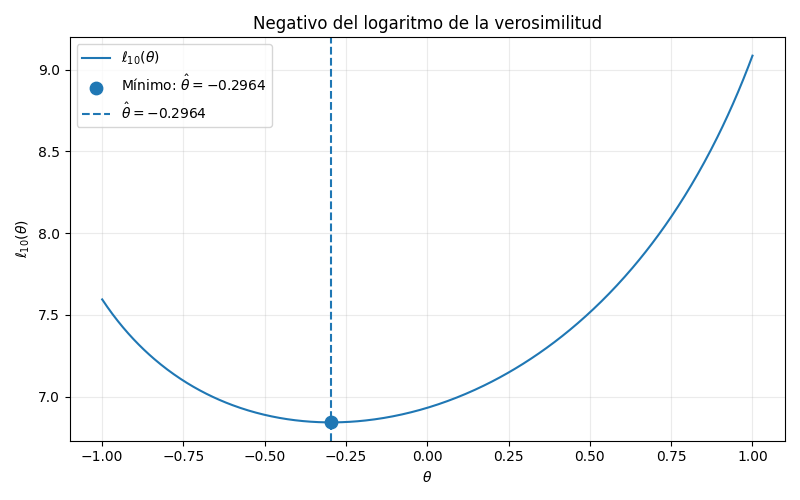
\includegraphics[width=0.8\textwidth]{../Imagenes/Prob1-2.png}



\begin{table}[htbp]
  \centering
  \caption{Estimaciones de $\hat{\theta}$ para 50 muestras y resultados del estimador.}
  \label{tab:estimaciones_theta_p1_3}
  
  \vspace{0.2cm}
  
  % Tabla de Estimaciones distribuidas en dos columnas
  \begin{tabular}{cc @{\hspace{1cm}} cc}
    \toprule
    \textbf{Muestra} & $\hat{\theta}$ & \textbf{Muestra} & $\hat{\theta}$ \\
    \midrule
    Muestra 1  & $-0.6984$ & Muestra 26 & $-0.9454$ \\
    Muestra 2  & $-0.2729$ & Muestra 27 & $\phantom{-}0.1093$ \\
    Muestra 3  & $-0.3693$ & Muestra 28 & $\phantom{-}0.0018$ \\
    Muestra 4  & $-0.3919$ & Muestra 29 & $\phantom{-}0.0331$ \\
    Muestra 5  & $-0.0140$ & Muestra 30 & $-0.1948$ \\
    Muestra 6  & $-1.0000$ & Muestra 31 & $\phantom{-}0.7936$ \\
    Muestra 7  & $\phantom{-}0.2042$ & Muestra 32 & $\phantom{-}0.0874$ \\
    Muestra 8  & $-0.6719$ & Muestra 33 & $-0.5961$ \\
    Muestra 9  & $-0.7925$ & Muestra 34 & $-0.6011$ \\
    Muestra 10 & $\phantom{-}0.0624$ & Muestra 35 & $-0.6111$ \\
    Muestra 11 & $-0.5335$ & Muestra 36 & $-0.7208$ \\
    Muestra 12 & $-0.2879$ & Muestra 37 & $-0.6421$ \\
    Muestra 13 & $\phantom{-}0.1988$ & Muestra 38 & $\phantom{-}0.5789$ \\
    Muestra 14 & $-0.2761$ & Muestra 39 & $-0.2544$ \\
    Muestra 15 & $-0.0860$ & Muestra 40 & $-0.2991$ \\
    Muestra 16 & $\phantom{-}0.0429$ & Muestra 41 & $\phantom{-}0.0013$ \\
    Muestra 17 & $-0.3404$ & Muestra 42 & $\phantom{-}0.1138$ \\
    Muestra 18 & $-0.4242$ & Muestra 43 & $-0.8044$ \\
    Muestra 19 & $\phantom{-}0.4641$ & Muestra 44 & $\phantom{-}0.4509$ \\
    Muestra 20 & $-0.3220$ & Muestra 45 & $-0.9042$ \\
    Muestra 21 & $-1.0000$ & Muestra 46 & $-0.0383$ \\
    Muestra 22 & $-1.0000$ & Muestra 47 & $-1.0000$ \\
    Muestra 23 & $-0.7742$ & Muestra 48 & $\phantom{-}0.8589$ \\
    Muestra 24 & $-0.2740$ & Muestra 49 & $-0.5412$ \\
    Muestra 25 & $-0.3749$ & Muestra 50 & $-0.6885$ \\
    \bottomrule
  \end{tabular}

  \vspace{0.4cm}

  % Tabla de Métricas de Resumen
  \begin{tabular}{ccccc}
    \toprule
    $\boldsymbol{\theta}$ \textbf{Verdadero} & \textbf{Media} ($\bar{\hat{\theta}}$) & \textbf{Sesgo} & \textbf{Varianza} & \textbf{ECM (MSE)} \\
    \midrule
    $-0.3333$ & $-0.2949$ & $0.0385$ & $0.2166$ & $0.2181$ \\
    \bottomrule
  \end{tabular}
\end{table}


% --- Bibliografía ---
\nocite{*}

\bibliographystyle{IEEEtran}
\bibliography{referencias}
\end{document}